\section{项目流程设计}
对于该项目,主要流程有四个分支,分别是治未病理论支撑、治未病在社区卫生建设的应用、问卷设计和实际调研。本项目旨在将治未病理论依照知信行模式应用于社区的卫生保健上以提高居民的健康水平。

因此理论设计中医治未病理论、卫生保健制度和知信行模式。之后就是探讨治未病相关的内容哪些可以和社区卫生保健建设相结合,可以分为内容上的,形式上的,政策支持后的实施情况等等。在这方面还特别需要对人群进行区分,健康群体/疾病人群;年轻受众/老年受众等等的差异可能让这些方面的差异变得很大。

接下来是设计问卷的阶段,由中医专业的同学完成初步的条目设计,以及参照陈建伟对于中医社区调查的研究。然后提交给相关的专家老师进行筛选,结合老师给出的筛查建议来确定最终的条目。

接下来是实际调研阶段,预计在暑假完成,两个月的时间,主要是发放问卷,之后经过一段时间的间隔,做一次重测也是够的。如果时间紧还可以在开学后接着完成。调研方式是发放问卷,为了追踪调查对象的情况,应该是挨家挨户的拜访,还可以就部分人群抽样做一些访谈以积累更多的调研资料。

其中一个问题是社区的选取,应该遵循随机分布的原则。另外,江宁区有中医药特色社区,可以选为对照组。这样其他的社区作为空白组,来进行结果上的对比。之后和社区方面联系来确认最后的有效率的发放方式。

最后就是分析收集来的数据,完成论文阶段最后的写作。对于挑战杯而言还涉及各种展示等等,对于各个环节都应该拍摄相关的照片和做好相应的记录,以便于答辩的进行。

\begin{figure}[th]
	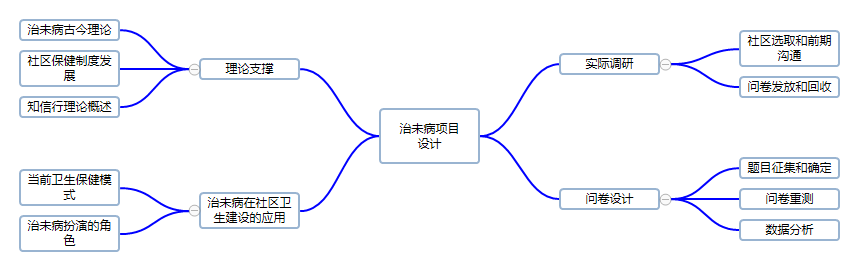
\includegraphics[width=\textwidth]{process.png}
	\centering
	\caption{项目设计简图}
\end{figure}